\documentclass[a4paper,12pt]{report}

% Packages
\usepackage{graphicx}
\usepackage{amsmath}
\usepackage{geometry}
\usepackage{fancyhdr}
\usepackage{setspace}
\usepackage{titlesec}  % For title formatting
\usepackage{hyperref}
\usepackage{xcolor}
\graphicspath{ {./images/} }

\usepackage[Lenny]{fncychap}
\ChNameUpperCase
\ChNumVar{\fontsize{40}{42}\usefont{OT1}{ptm}{m}{n}\selectfont}
\ChTitleVar{\Large\sc}

\geometry{margin=1in}
\setstretch{1.5}

\usepackage{listings}

\definecolor{codegreen}{rgb}{0,0.6,0}
\definecolor{codegray}{rgb}{0.5,0.5,0.5}
\definecolor{codepurple}{rgb}{0.58,0,0.82}
\definecolor{backcolour}{rgb}{0.95,0.95,0.92}

\lstdefinestyle{mystyle}{
    backgroundcolor=\color{backcolour},   
    commentstyle=\color{codegreen},
    keywordstyle=\color{magenta},
    numberstyle=\tiny\color{codegray},
    stringstyle=\color{codepurple},
    basicstyle=\ttfamily\footnotesize,
    breakatwhitespace=false,         
    breaklines=true,                 
    captionpos=b,                    
    keepspaces=true,                 
    numbers=left,                    
    numbersep=5pt,                  
    showspaces=false,                
    showstringspaces=false,
    showtabs=false,                  
    tabsize=2
}

\lstset{style=mystyle}



% Header and Footer
\pagestyle{fancy}
\fancyhf{}
\fancyhead[L]{OverseerAI}
\fancyhead[R]{\thepage}

% Title Formatting
\titleformat{\section}{\normalfont\Large\bfseries}{\thesection}{1em}{}


% Cover Page
\title{
    
\includegraphics[width=0.40\textwidth]{images/logo_overseerai.png}
    
    \textbf{\Huge OverseerAI} \\
    \vspace{1cm} % Adjust vertical space
    \large Laurea di Informatica L-31 all'Università di Salerno \\
    \large Corso di Fondamenti di Intelligenza Artificiale \\
    \vspace{0.5cm} % Adjust vertical space
    \small \textit{Gennaio 2025} \\
    \vspace{3cm}
    \textbf{Created by: }{\large Antonio Maiorano} \\
    \vspace{0.5cm}
    \textbf{Supervised by: }{\large Prof. Fabio Palomba}
}
\date{}

\tolerance=1
\emergencystretch=\maxdimen
\hyphenpenalty=10000
\hbadness=10000

\begin{document}

% Title Page
\maketitle
\thispagestyle{empty}
\newpage

% Table of Contents
\renewcommand*\contentsname{\hfill Indice \hfill}
% Start page numbering from the Table of Contents
\setcounter{page}{1}  % Start counting from 1
\tableofcontents
\newpage

\begingroup%
\makeatletter%
\let\clearpage\relax% Stop LaTeX from going to a new page; and
\vspace*{\fill}%
\vspace*{\dimexpr-50\p@-\baselineskip}% Remove the initial (default) 50pt gap (plus 1 line)
\chapter{Definizione del problema}
\vspace*{\fill}%
\endgroup
\newpage


\section{Introduzione}
YouTube è una delle piattaforme di condivisione video più utilizzate al mondo. Tuttavia, con l'aumento dei contenuti, sono cresciuti anche i tentativi di truffa, certe volte mascherati con il metodo "\textit{fare tanto, dando poco}".\\
Per semplicità di analisi, i contenuti "truffa" sono una generalizzazione di tutti quei contenuti che portano l'utente finale a consumare contenuti che sono descritti in modo fuorviante e/o sbagliato, si includono dunque i contenuti che reindirizzano ad altri contenuti esterni alla piattaforma per lo stesso obiettivo.\\
Queste problematiche sono ora piu' presenti che mai a causa della rapida crescita della presenza online dei contenuti AI-Made (le cosiddette "Money Farm") e pubblicità sponsorizzate da individui singoli con intenzioni a volte poco chiare, e poco legittime.

\section{Obiettivi}
L'obiettivo principale di questo progetto è quello di evitare il piu' possibile un contatto diretto con questi contenuti-truffa creando un modello di Machine Learning in grado di classificare i titoli dei video.

\section{Specifica P.E.A.S.}
\subsection{Performance}
La misura delle prestazioni del modello:
\begin{itemize}
    \item Correttezza di classificazione dei titoli.
\end{itemize}

\subsection{Environment}
Descrizione degli elementi che formano l'ambiente in cui il modello opererà:
\begin{itemize}
    \item Dataset sintetico di titoli creati con l'aiuto di Large Language Models, i cui elementi saranno descritti di seguito (applicati limiti derivanti dalla piattaforma stessa).
\end{itemize}

\subsection{Actuators}
Gli attuatori che prenderanno le decisioni nel modello:
\begin{itemize}
    \item Classificatore che determinerà l'appartenenza di un titolo ad una delle due categorie.
\end{itemize}

\subsection{Sensors}
I sensori attraverso cui il modello riceve le percezioni su cui opererà:
\begin{itemize}
    \item La finestra di input.
\end{itemize}

\section{Caratteristiche dell'Ambiente}
\begin{itemize}
    \item \textbf{Osservabilità:} Parzialmente osservabile.
    \begin{itemize}
        \item Il modello può osservare ed analizzare solo le caratteristiche del video e non il contenuto del video stesso.
    \end{itemize}
    \item \textbf{Determinismo:} Parzialmente stocastico.
    \begin{itemize}
        \item Presenza di ambiguità e rumore all'interno delle caratteristiche in analisi.
    \end{itemize}
    \item \textbf{Episodicità:} Episodico.
    \begin{itemize}
        \item Ogni titolo viene esaminato indipendentemente dagli altri
    \end{itemize}
    \item \textbf{Dinamismo:} Statico.
    \begin{itemize}
        \item I dati usati dal modello sono costanti, e non subiscono cambiamenti.
    \end{itemize}
    \item \textbf{Tipo di agente:} Singolo agente.
    \begin{itemize}
        \item Vi è un solo agente ad analizzare i titoli.
    \end{itemize}
\end{itemize}

\newpage

\section{Metodologia}
La valutazione della metodologia di approccio al problema in analisi è stata fatta tra i modelli di Ingegneria del Machine Learning \textbf{CRISP-DM} e \textbf{TDSP}, dove è stato scelto il primo, data la non necessità di suddivisioni e validazioni temporali del progetto presenti nel secondo.

\subsection{CRISP-DM}
Le fasi che verranno percorse sono:
\begin{enumerate}
    \item Business Understanding.
    \item Data Understanding.
    \item Data Preparation.
    \item Data Modeling.
    \item Evaluation.
\end{enumerate}

\newpage

\begingroup%
\makeatletter%
\let\clearpage\relax% Stop LaTeX from going to a new page; and
\vspace*{\fill}%
\vspace*{\dimexpr-50\p@-\baselineskip}% Remove the initial (default) 50pt gap (plus 1 line)
\chapter{Business Understanding}
\vspace*{\fill}%
\endgroup
\newpage

\section{Determinare gli Obiettivi di Business}
Il primo passo per la creazione di OverseerAI, è capire cosa esso deve essere, come deve esserlo e come esso deve arrivare ad essere cio' che è stato descritto di esso.
\subsection{Background}
Esistono molti sistemi di "Auto-Flagging", o di Moderazione automatica, YouTube stesso ne ha almeno uno!\\
...Il problema è che i contenuti moderati sono solo quelli degli utenti, ad esempio le pubblicità non sono moderate, per qualche ragione di Business di Google.\\
Un sistema esistente (e dignitosamente più funzionante dell'esempio appena esplicitato) da cui OverseerAI potrebbe prendere spunto:
\begin{itemize}
    \item \textbf{La moderazione automatica del social media TikTok} 
\end{itemize}
Il suddetto sistema funziona sulla base di un algoritmo (Closed-Source) che modera i contenuti in modo automatico basandosi su similarità con i contenuti di allenamento, che, nel caso di TikTok, possono essere Hashtags riconosciuti come pericolosi (la ricerca sulla piattaforma di tali Hashtags porta zero risultati), oppure delle parole presenti nella descrizione che sono anche essere già conosciute come pericolose.\\
Con grande probabilità esso utilizza anche un algoritmo per l'analisi dei contenuti.\\
A prescindere dall'algoritmo, TikTok blocca i contenuti ben prima che siano caricati, e nel caso dei contenuti sponsorizzati, essi vengono controllati allo stesso modo dei contenuti degli utenti normali.

\subsection{Obiettivi di Business}
Basandoci sulle informazioni raccolte, OverseerAI dovrà analizzare TUTTI i contenuti di YouTube, in particolare i loro titoli. Assieme ad essi si potrebbe analizzare la presenza di link all'interno della descrizione, che sono la maggior parte delle volte usati per truffare e rubare dati alle persone ignare.\\
Ovviamente quest'ultimo puo' facilmente essere un falso positivo, in quanto ci sono anche canali leciti che usano i link per aiutare le persone a connettere con loro attraverso altri social media.

\newpage
\section{Criteri di successo}
Gli obiettivi, non per ordine di importanza, di OverseerAI dunque sono:
\begin{itemize}
    \item \textbf{Un corretto riconoscimento dei contenuti intenzionati a truffare}
    \item \textbf{Un corretta classificazione dei contenuti normali come leciti}
    \item \textbf{Evitare di creare bias con chi ha link nei propri contenuti}
\end{itemize}
Ovviamente, assieme ad essi, c'è anche il criterio di aver sventato delle truffe!

\section{Limiti}
A causa di un recente cambiamento nella piattaforma di Youtube, vi è un limite alla consumazione di contenuti, soprattutto se l'utente non ha eseguito il Login.\\
Inoltre, anche lo scraping stesso del sito è stato limitato di molto (\href{https://web.archive.org/web/20240807161716/https://www.tomsguide.com/ai/nvidia-accused-of-scraping-80-years-worth-of-of-videos-daily-to-train-ai-models-what-you-need-to-know}{\color{blue}{causa}}).\\
Volendo evitare un aumento esponenziale della complessità del progetto, dovuto anche al dover ricercare manualmente le entries da aggiungere al dataset, e volendo rimanere in un'ottica più generale, l'intenzione iniziale di usare dati reali ottenuti dalla piattaforma stessa è stata accantonata,  ai dati creati sinteticamente tramite l'uso di LLMs e tramite l'utilizzo di scripts python di potenziamento.

\section{Tecnologie Usate}
Le principali tecnologie usate sono:
\begin{itemize}
    \item I \textbf{LLMs} come tool di supporto;
    \item \textbf{Python} come linguaggio di programmazione;
    \begin{itemize}
        \item Diverse librerie usate per le funzioni critiche, tra le quali \texttt{\color{red}{pandas}} per alcune funzioni base eseguite sul Dataset, \texttt{\color{red}{sklearn}} per le funzioni di Machine Learning, etc...
    \end{itemize}
\end{itemize}

\newpage

\begingroup%
\makeatletter%
\let\clearpage\relax% Stop LaTeX from going to a new page; and
\vspace*{\fill}%
\vspace*{\dimexpr-50\p@-\baselineskip}% Remove the initial (default) 50pt gap (plus 1 line)
\chapter{Data Understanding}
\vspace*{\fill}%
\endgroup
\newpage

\section{Ottenimento dei Dati}
Come descritto in precedenza, a causa di alcuni limiti non ci sarà possibile utilizzare dati reali.\\
Al loro posto, utilizzeremo dei dati creati sinteticamente tramite l'uso di LLMs.\\
Dopo l'istruzione, del suddetto, a riguardo del problema in esame, e del contesto ad esso relativo, non vi è granchè bisogno di fare Prompt Engineering: richiedendo semplicemente la generazione delle istanze, e per ogni iterazione essere sicuri di non averne di ripetute per evitare problemi, esso ne genererà continuamente.\\
Le istanze generate sono istanze di struttura CSV, dove vi sono solo due features:
\begin{itemize}
        \item Il \textbf{titolo}, \texttt{\color{red}{title}};
        \item Una \textbf{etichetta, Target Feature del dataset}, \texttt{\color{red}{label}}, che può essere "scam" o "legit", e determina se un video è truffaldino o meno;
        \item Una \textbf{descrizione}, \texttt{\color{red}{description}}, che contiene testo e può contenere link al suo interno.
\end{itemize}
Le istanze sono generate solo con queste tre features causa la tipologia delle features stesse: sono strettamente collegate e devono avere senso nel contesto dell'istanza, dunque non possono essere generate come le altre features, invece indipendenti tra loro.\\
Inoltre le istanze verranno generate in inglese per semplicità.

\section{Miglioramento del Dataset}
\subsection{Aggiunta di features}
I dati creati sinteticamente mancano di alcune features collegate ai contenuti.\\
Ovviamo a questo problema creando da zero dei dati realistici, con funzioni randomiche basate su osservazioni soggettive dei casi reali.\\
Le features riguardante i contenuti che verranno create sono:
\begin{itemize}
        \item I \textbf{mi piace} come \texttt{\color{red}{likes}};
        \item I \textbf{non mi piace} come \texttt{\color{red}{dislikes}};
        \item L' \textbf{ora di caricamento} come \texttt{\color{red}{upload\_hour}};
        \item I \textbf{commenti} come \texttt{\color{red}{comments}}.
\end{itemize}
Dopo aver creato le features nel dataset, procederemo ad assegnare ad ogni istanza dei valori ad essi riguardanti.\\

\begin{lstlisting}[language=Python]
import pandas as pd
import random
import numpy as np

def add_features(df):
    df['upload_hour'] = np.random.randint(0, 24, df.shape[0])
    df['likes'] = np.random.randint(0, 100001, df.shape[0])
    df['dislikes'] = np.random.randint(0, 10001, df.shape[0])
    df['comments'] = np.random.randint(0, 10001, df.shape[0])
\end{lstlisting}

\subsection{Aggiunta di rumore}
Il dataset risultante è vicino ad alla realtà, ma per renderlo ancor più realistico aggiungiamo del rumore nei dati, molto spesso presente in qualsiasi dataset.\\
Per il 3\% delle istanze del dataset, viene introdotto rumore per la feature "titolo", e la tipologia di rumore viene introdotto randomicamente nella scelta di uno dei seguenti:
\begin{itemize}
        \item Sostituzione di caratteri con caratteri casuali;
        \item Aggiunta di caratteri speciali;
        \item Mescolamento dei caratteri originali;
        \item Testo generico di errore.
\end{itemize}
Per il 5\% delle istanze del dataset, viene introdotto rumore per una delle features tra "upload\_hour", "likes", "dislikes" o "comments", immettendo valori vuoti "NaN".\\
Per il 5\% delle istanze del dataset, viene introdotto rumore per le features "likes" e "dislikes" immetendo valori anomali, in questo caso valori assurdi.
\\
\begin{lstlisting}[language=Python]
import pandas as pd
import random
import numpy as np
def add_noise(df):
    def corrupt_title(title):
        if pd.isnull(title):
            return title

        noise_methods = [
            lambda x: ''.join(random.choice(string.ascii_letters + string.digits + string.punctuation) for _ in range(len(x))),
            lambda x: x + ''.join(random.choices(string.punctuation, k=5)), 
            lambda x: ''.join(random.sample(x, len(x))),
            lambda x: '###ERROR###'
        ]

        return random.choice(noise_methods)(title)

    noise_indices = df.sample(frac=0.03).index
    df.loc[noise_indices, 'title'] = df.loc[noise_indices, 'title'].apply(corrupt_title)

    for col in ['upload_hour', 'likes', 'comments']:
        df.loc[df.sample(frac=0.05).index, col] = np.nan

    noise_indices = df.sample(frac=0.05).index
    (`len(noise_indices)`)
    df.loc[noise_indices, 'likes'] = np.random.randint(1000000, 10000000, len(noise_indices))
    df.loc[noise_indices, 'dislikes'] = np.random.randint(500000, 1000000, len(noise_indices))

    return df
\end{lstlisting}
\newpage

\begingroup%
\makeatletter%
\let\clearpage\relax% Stop LaTeX from going to a new page; and
\vspace*{\fill}%
\vspace*{\dimexpr-50\p@-\baselineskip}% Remove the initial (default) 50pt gap (plus 1 line)
\chapter{Data Preparation}
\vspace*{\fill}%
\endgroup
\newpage

\section{Preparazione del dataset}
Il dataset in uso presenta tipi diversi di rumore: su tutte le features, ci sono dei valori anomali che potrebbero creare problematiche anche rilevanti durante la creazione e l'utilizzo del modello.\\
Prima di passare dunque alla suddetta fase, il dataset deve essere pulito.\\
Inoltre, i valori numerici potrebbero essere problematici in fase di training, in quanto risulta avere valori senza un contesto: un esempio semplice può essere \texttt{\color{red}{upload\_hour}} che è un valore numerico con un contesto specifico, ovvero quello delle ore in una giornata, e non ha dunque senso unicamente come numero e fuori contesto.\\
Infine, i testi, nella forma attuale, devono essere normalizzati per avere una forma non ambigua e facilitare la fase di training.

\section{Data cleaning}
\subsection{Valori numerici}
Le prime features del processo di pulizia sono \texttt{\color{red}{upload\_hour}}, \texttt{\color{red}{likes}}, \texttt{\color{red}{dislikes}} e \texttt{\color{red}{comments}}.\\
In esse, abbiamo due problematiche principali:
\begin{itemize}
        \item La presenza di valori mancanti;
        \item La presenza di valori assurdi/anomali.
\end{itemize}
La prima problematica si risolve con una semplice \textbf{Imputazione statistica}, usando come funzione la Mediana.
\begin{lstlisting}[language=Python]
import pandas as pd
import re
# ...NLP libraries
def clean_dataset(df):
    def value_imputation(df, column):
        median_value = df[column].median()
        df[column].fillna(median_value, inplace=True)
        return df
    for col in ['upload_hour', 'likes', 'dislikes', 'comments']:
        df = value_imputation(df, col)
\end{lstlisting}
La seconda problematica si risolve utilizzando una funzione statistica di \textbf{Range Interquartile} (IQR), i valori in analisi che non rispettano il suddetto vengono rimpiazzati con il valore mediano della colonna in cui esso si trova.
\\
\[
\text{IQR} = Q_3 - Q_1
\]
\[
\textbf{dove}
\]
\[
Q_1 = \text{termine in posizione } \frac{n + 1}{4}
\]
\[
Q_3 = \text{termine in posizione } \frac{3(n + 1)}{4}
\]
\begin{figure}[h]
\centering
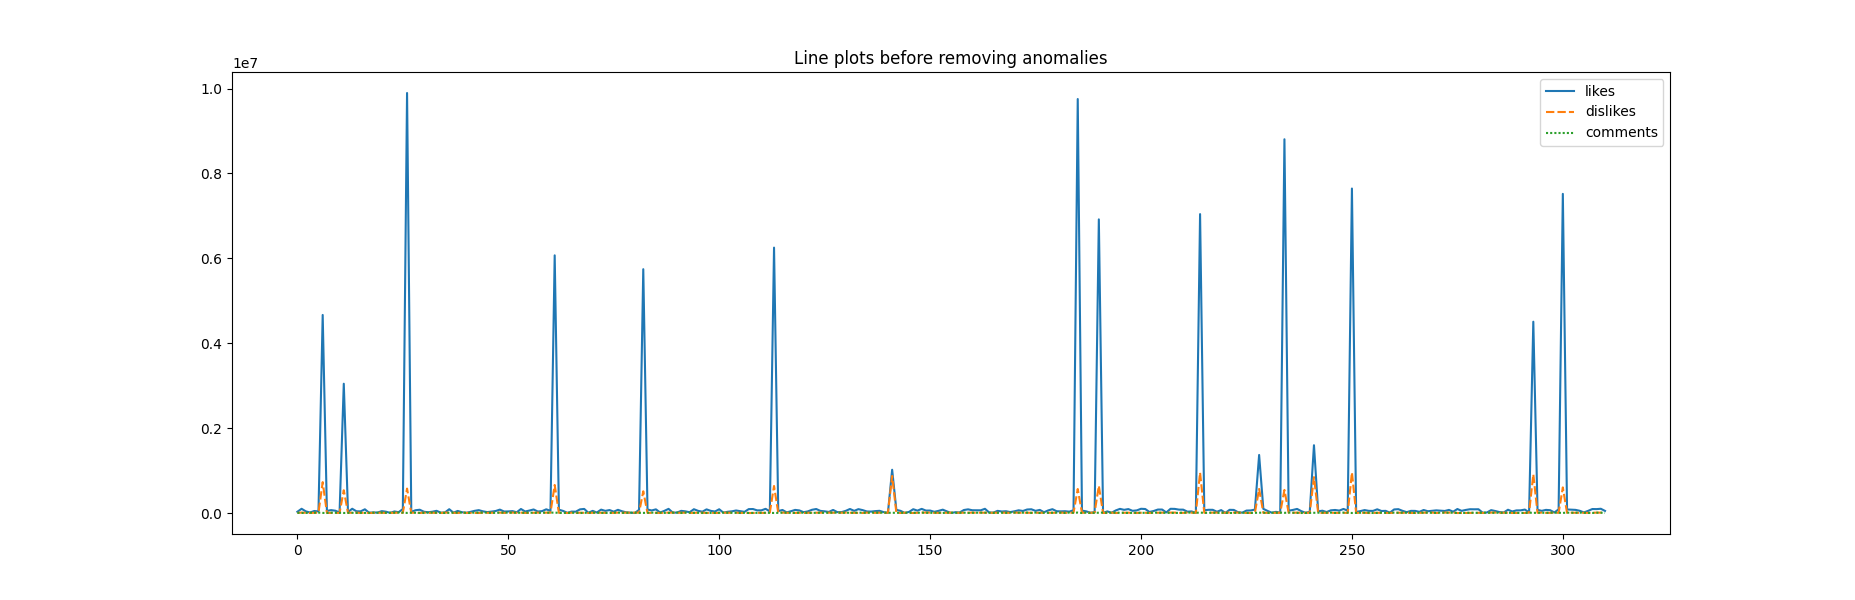
\includegraphics[width=\textwidth]{before_IQR.png}
\caption{Prima della rimozione degli Outliers (anomalie)}
\end{figure}
\begin{figure}[h]
\centering
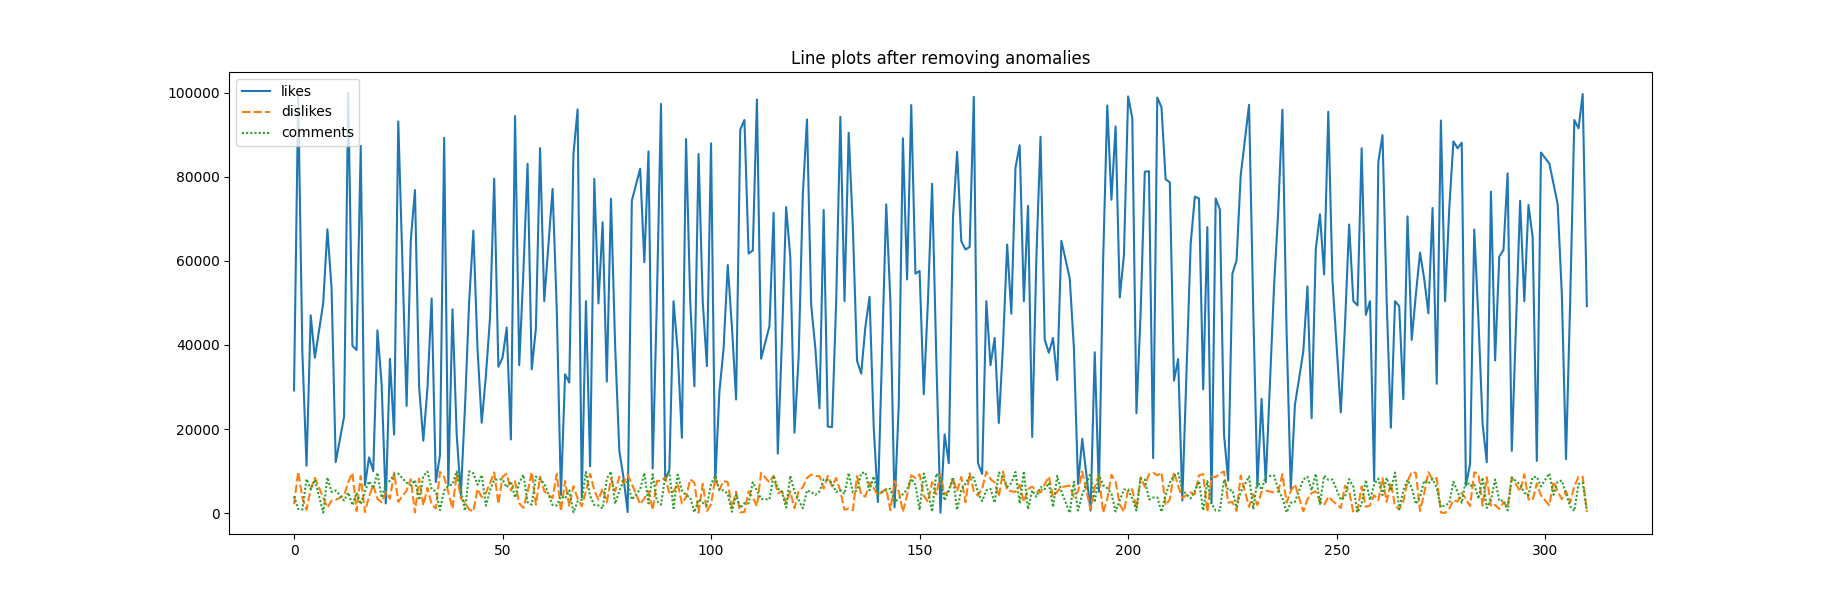
\includegraphics[width=\textwidth]{after_IQR.png}
\caption{Dopo la rimozione degli Outliers (anomalie)}
\end{figure}
\newpage
\begin{lstlisting}[language=Python]
import pandas as pd
import re
import nltk
from nltk.corpus import stopwords
from nltk.stem import WordNetLemmatizer
from nltk.tokenize import word_tokenize
from spellchecker import SpellChecker
from num2words import num2words

def clean_dataset(df):
    # ...
    def remove_anomalies(df, column):
        Q1 = df[column].quantile(0.25)
        Q3 = df[column].quantile(0.75)
        IQR = Q3 - Q1
        lower_bound = Q1 - 1.5 * IQR
        upper_bound = Q3 + 1.5 * IQR
        median_val = df[column].median()
        df.loc[df[column] < lower_bound, column] = median_val
        df.loc[df[column] > upper_bound, column] = median_val
        return df
    for col in ['likes', 'dislikes', 'comments']:
        df = remove_anomalies(df, col)
\end{lstlisting}
\subsection{Valori testuali}
Le successive features soggette al processo di pulizia sono le feature testuali, ovvero \texttt{\color{red}{title}} e \texttt{\color{red}{description}}.\\
In esse abbiamo 5 problematiche principali:
\begin{itemize}
        \item La presenza di valori di errore ("\#\#\#ERROR\#\#\#");
        \item La presenza di caratteri speciali;
        \item Titolo non normalizzato;
        \item La presenza di links (solo \texttt{\color{red}{description}});
        \item La presenza di valori corrotti (solo \texttt{\color{red}{title}}).
\end{itemize}
La prima problematica (valori di errore) è risolvibile facilmente, eseguendo un parsing con le istanze che rispettano il criterio di eguaglianza con la stringa:
\begin{lstlisting}[language=Python]
import # ...

def clean_dataset(df):
    # ...
    def clean_title(title):
        if pd.isnull(title) or '###ERROR###' in str(title):
            return "Title Not Available"
\end{lstlisting}

La seconda problematica (caratteri speciali) è ancor piu' facile da risolvere, rimuovendo semplicemente i caratteri speciali utilizzando delle \textbf{Regular Expression}.
\begin{lstlisting}[language=Python]
import # ...

def clean_dataset(df):
    # ...
    def clean_title(title):
        # ...
        title = re.sub(r'[^\w\s]', '', str(title))
        title = re.sub(r'\s+', ' ', title).strip()
\end{lstlisting}
La prima REGEX serve a eliminare i caratteri speciali, la seconda elimina gli spazi quando ce ne sono più di uno.\\
\\
Successivamente viene eseguita l'eliminazione delle istanze corrotte riconosciute fino a questo punto.
\begin{lstlisting}[language=Python]
import # ...

def clean_dataset(df):
    # ...
    def clean_title(title):
        # ...
        
    df = df[df['title'] != "Title Not Available"]
\end{lstlisting}
\newpage

La terza problematica (titolo non normalizzato) si può risolvere seguendo delle regole standard per la normalizzazione del testo. In questo caso sono state praticate:
\begin{itemize}
        \item Contraction Expansion;
        \item Tokenizzazione;
        \item Conversione dei numeri (in cifre) in parole;
        \item Lemmatizzazione;
        \item Trasformazione in Minuscolo;
        \item Stopword Removal.
\end{itemize}
\begin{lstlisting}[language=Python]
import # ...

def clean_dataset(df):
    # ...
    def normalize_title(title):
        if not isinstance(title, str):
            print(f"Titolo non valido: {title}")
            return None

        try:
            contractions = {
                "I'm": "I am", "you're": "you are", "he's": "he is",
                "she's": "she is", "it's": "it is", "we're": "we are",
                "they're": "they are", "can't": "cannot",
                "won't": "will not", "don't": "do not",
                "didn't": "did not","isn't": "is not",
            }
            for contraction, full_form in contractions.items():
                title=re.sub(r'\b'+contraction+r'\b',full_form,title)

            tokens = word_tokenize(title)

            tokens = [
                num2words(word) if word.isdigit() else word
                for word in tokens
            ]

            tokens=[lemmatizer.lemmatize(word) for word in tokens if word]

            tokens = [word.lower() for word in tokens]

            tokens=[word for word in tokens if word not in stop_words]

            normalized_title = ' '.join(tokens)

            return normalized_title if normalized_title.strip() else None
        except Exception as e:
            print(f"Errore durante la normalizzazione del titolo: {title}. Errore: {e}")
            return None
\end{lstlisting}
Anche qui si controlla se il titolo risultante è vuoto, e nel caso si elimina la riga corrispondente.
\\
\\
La quarta problematica (presenza di links in \texttt{\color{red}{description}}) è risolvibile anche essa usando una semplice Regular Expression.
\\
Essendo il link, inoltre, l'unico elemento del campo effettivamente rilevante, possiamo procedere ad estrarre solo esso dal valore attuale.
\begin{lstlisting}[language=Python]
import # ...

def clean_dataset(df):
    # ...
    def process_description(description):
        link = re.search(r'http[s]?://\S+', description)
        return link.group() if link else "No link available"
\end{lstlisting}
\newpage
La quinta problematica (valori corrotti) invece può essere risolta solo manualmente, non esiste un sistema automatico funzionante al 100\% in quanto i valori corrotti sono di natura totalmente casuale.\\
Andiamo dunque a eliminare istanze del nuovo dataset risultato dalle precedenti operazioni che contengono valori corrotti. Dall'osservazione fatta, risultano essere i seguenti (elencati per titolo):
\begin{itemize}
    \item "pqjjlbwwsupivcnmfi9i2m8jtdw"
    \item "son0mmgo6vr2rbo6ixhnjnvvem2r8qc"
\end{itemize}

\end{document}
